\documentclass[10pt,a4paper,titlepage]{article}
\usepackage[a4paper,top=2.5cm,bottom=2.5cm,left=2.5cm,right=2.5cm]{geometry}
%\usepackage{scicite}
\usepackage{times}
\usepackage{hyperref}
\usepackage{setspace}
\usepackage{amsmath}
\usepackage{listings}
\usepackage{graphicx}


\makeatletter
\renewcommand*\env@matrix[1][*\c@MaxMatrixCols c]{%
  \hskip -\arraycolsep
  \let\@ifnextchar\new@ifnextchar
  \array{#1}}
\makeatother

%\topmargin 0.0cm
%\oddsidemargin 0.2cm
%\textwidth 16cm 
%\textheight 21cm
%\footskip 1.0cm

%The next command sets up an environment for the abstract to your paper.

\newenvironment{sciabstract}{%
\begin{quote} \bf}
{\end{quote}}


% If your reference list includes text notes as well as references,
% include the following line; otherwise, comment it out.

%\renewcommand\refname{References}

% The following lines set up an environment for the last note in the
% reference list, which commonly includes acknowledgments of funding,
% help, etc.  It's intended for users of BibTeX or the {thebibliography}
% environment.  Users who are hand-coding their references at the end
% using a list environment such as {enumerate} can simply add another
% item at the end, and it will be numbered automatically.




% Include your paper's title here

\title{FYS4150 Project 2} 
\author
{Mikkel Killingmoe Christensen\\
\\
\normalsize{\today}
}

% Include the date command, but leave its argument blank.

\date{}

%%%%%%%%%%%%%%%%% END OF PREAMBLE %%%%%%%%%%%%%%%%



\begin{document} 

% Double-space the manuscript.

\baselineskip24pt

% Make the title.

\maketitle 
\begin{center}
\par GitHub repository:
\par \url{https://github.com/mikkello/FYS4150/}
\end{center}


% Place your abstract within the special {sciabstract} environment.

\begin{center}
{\large \textbf{Abstract}}
\end{center}
\begin{sciabstract}
Eigenvalue problems are common in natural science, but they are often impossible to solve analytically. It is thus important to develop fast and reliable numerical solvers. In this project, an eigenvalue solver based on Jabobi's algorithm was programmed in C++ to solve the Schroedinger equation for electrons in a harmonic oscillator. Different number of grid points, approximations of the boundary condition and frequencies in the algorithm were investigated. It was found that the choice of these values greatly influenced computation time and accuracy. It was also found that the algorithm had a considerably longer computation time than the Armadillo solver.  
\end{sciabstract}



\section{Introduction}
Eigenvalue problems are common in many areas of physics and chemistry. They can, however, be difficult or impossible to solve analytically for large systems. It is thus natural to develop algorithms to solve these problems numerically. The goal of this project is to develop an algorithm that uses Jacobi's method for finding eigenvalues. It will then be used to solve the Schroedinger equation for one or two electrons in a three-dimensional harmonic oscillator well. The results can potentially be used to study so-called quantum dots, which is a hot topic in solid-state physics.


\section{Theory}
\subsection{Schroedinger's equation for one electron}
The first goal will be to solve the radial part of Schroedinger's equation (SE) for one electron in a three-dimensional harmonic oscillator well. Spherical symmetry is assumed. The equation that follows (\ref{eq:SL1})is the Schroedinger equation that needs to be solved, and it will in this section be simplified for easier implementation. The derivations in this project are base on the lecture notes of Morten Hjorth-Jensen [1].
\begin{equation}
\label{eq:SL1}
  -\frac{\hbar^2}{2 m} \left ( \frac{1}{r^2} \frac{d}{dr} r^2
  \frac{d}{dr} - \frac{l (l + 1)}{r^2} \right )R(r) 
     + V(r) R(r) = E R(r).
\end{equation} where $r\in[0,\infty)$ because of the transformation to spherical coordinates.
The potential for the harmonic oscillator is given by:
\begin{equation}
V(r) = \frac{1}{2}kr^{2}, k = m\omega^{2}
\end{equation}
By assuming $l=0$, the energies are given by:
\begin{equation}
\label{eq:energy1}
E_{nl}=  \hbar \omega \left(2n+l+\frac{3}{2}\right),
\end{equation}
with $n=0,1,2,\dots$ and $l=0,1,2,\dots$.
Substituting $R(r)=(1/r)u(r)$ in equation (\ref{eq:SL1}) and assuming $l=0$, yields the following equation:
\begin{equation}
\label{eq:SL2}
  -\frac{\hbar^2}{2 m} \frac{d^2}{dr^2} u(r) 
       + V(r)u(r)  = E u(r) .
\end{equation}
A dimensionless variable $\rho=r/ \alpha$ is now introduced. This changes the potential to $V(\rho)=k\alpha^{2}\rho^{2}/2$. Inserting the new variable and the potential into equation (\ref{eq:SL2}), yields:
\begin{equation}
\label{eq:SL3}
  -\frac{d^2}{d\rho^2} u(\rho) 
       + \frac{mk}{\hbar^2} \alpha^4\rho^2u(\rho)  = \frac{2m\alpha^2}{\hbar^2}E u(\rho) .
\end{equation}
By defining $\alpha$ through:
\begin{equation}
\dfrac{mk\alpha^{4}}{\hbar^{2}}=1,
\end{equation}
and also defining
\begin{equation}
\lambda = \frac{2m\alpha^2}{\hbar^2}E,
\end{equation}
Schroedinger's equation can now be written as:
\begin{equation}
\label{eq:SL4}
  -\frac{d^2}{d\rho^2} u(\rho) + \rho^2u(\rho)  = \lambda u(\rho).
\end{equation}
This is finally on a form that is easier to solve numerically.

By using Taylor expansion, it can be shown that the second derivative can be expressed as:
\begin{equation}
\label{eq:secondiff}
    u''=\frac{u(\rho+h) -2u(\rho) +u(\rho-h)}{h^2} +O(h^2),
\end{equation}
where $h$ is the step length. Using $n$ grid points, $\rho_{min}=\rho_{0}$ and $\rho_{max}=\rho_{n}$ the step length becomes\begin{equation}
\label{eq:steplength}
  h=\frac{\rho_n-\rho_0 }{n}.
\end{equation}
Equation (\ref{eq:SL4}) can be discretized with
\begin{equation}
\rho_i= \rho_0 + ih \ \ \ \ \ i=1,2,\dots , n,
\end{equation}
giving the discretized version:
\begin{equation}
\label{eq:SL_disc1}
-\frac{u_{i+1} -2u_i +u_{i-1} }{h^2}+V_iu_i  = \lambda u_i,
\end{equation}
where $V_{i}=\rho_{i}^{2}$ is the harmonic oscillator potential.
Finally, this equation can be written as a linear set of equations:
\begin{equation}
A\mathbf{u}=\lambda\mathbf{u}
\end{equation}
where A is the matrix
\setcounter{MaxMatrixCols}{20}
\begin{equation}
A=\begin{pmatrix}
\frac{2}{h^2} + V_1 && -\frac{1}{h^2} && 0 && ... && 0 && 0 \\
-\frac{1}{h^2} && \frac{2}{h^2} + V_2 && -\frac{1}{h^2} && ... && 0 && 0 \\
0 && -\frac{1}{h^2} && \frac{2}{h^2} + V_3 && ... && 0 && 0 \\
: && : && : && ^{\textbf{.}}. && : && : \\
0 && 0 && 0 && -\frac{1}{h^2} && \frac{2}{h^2} + V_{N-2} && -\frac{1}{h^2} \\
0 && 0 && 0 && 0 && -\frac{1}{h^2} && \frac{2}{h^2} + V_{N-1}.
\end{pmatrix}
\label{eq:A}
\end{equation}


\subsection{Schroedinger's equation for two electrons}
Two study the case where two electrons are trapped in the well, a new equation has to be set up. Repulsive Coulomb interaction will also be added. Without the repulsive interaction, the Schroedinger equation is given by:
\begin{equation}
\label{eq:SE5}
\left(  -\frac{\hbar^2}{2 m} \frac{d^2}{dr_1^2} -\frac{\hbar^2}{2 m} \frac{d^2}{dr_2^2}+ \frac{1}{2}k r_1^2+ \frac{1}{2}k r_2^2\right)u(r_1,r_2)  = E^{(2)} u(r_1,r_2) .
\end{equation}
The wave function now includes two r vectors and the two-electron energy $E^{(2)}$. It is convenient to work with relative coordinates, and therefore $\mathbf{r} = \mathbf{r}_1-\mathbf{r}_2$
and the center-of-mass coordinate $\mathbf{R} = 1/2(\mathbf{r}_1+\mathbf{r}_2)$ are introduced. Schrödinger's equation does now read:
\begin{equation}
\left(  -\frac{\hbar^2}{m} \frac{d^2}{dr^2} -\frac{\hbar^2}{4 m} \frac{d^2}{dR^2}+ \frac{1}{4} k r^2+  kR^2\right)u(r,R)  = E^{(2)} u(r,R).
\end{equation}
Now, the equation can be split in an $\mathbf{r}$ part and an $\mathbf{R}$ by writing the wave function as $u(r,R) = \psi(r)\phi(R)$. The energy can then be split up into the relative energy $E_{r}$ and the center-of-mass energy $E_{R}$. The total energy is then given by the sum of these two
\begin{equation}
\label{eq:totE}
E^{(2)}=E_{R}+E_{r}.
\end{equation}
Since the repulsive Coulomb interaction is included, a new interaction potential is needed. This is given by:
\begin{equation}
\label{eq:pot_co}
V(r_1,r_2) = \frac{\beta e^2}{|\mathbf{r}_1-\mathbf{r}_2|}=\frac{\beta e^2}{r},
\end{equation}
where $\beta e^2=1.44$ eVnm.
Including this in the Schroedinger equation gives the following:
\begin{equation}
\left(  -\frac{\hbar^2}{m} \frac{d^2}{dr^2}+ \frac{1}{4}k r^2+\frac{\beta e^2}{r}\right)\psi(r)  = E_r \psi(r).
\end{equation}
Again, the equation can be simplified by introducing a dimensionless variable $\rho=r/a$. Doing this, the equation becomes:
\begin{equation}
-\frac{d^2}{d\rho^2} \psi(\rho)+\frac{mk}{\hbar^2} \alpha^4\rho^2\psi(\rho)+\frac{m\alpha \beta e^2}{\rho\hbar^2}\psi(\rho)=\frac{m\alpha^2}{\hbar^2}E_r \psi(\rho).
\end{equation}
The goal is to make the equation similar to equation (\ref{eq:SL4}) which is suitable for numerical algorithms. This is again done by fixing $\alpha$, and also introducing a new frequency and a new energy term. 
\begin{equation*}
\frac{m\alpha \beta e^2}{\hbar^2}=1 \qquad  \omega_r^2 = \frac{mk\alpha^4}{4\hbar^2} \qquad \lambda = \frac{m\alpha^2E}{\hbar^2}.
\end{equation*}
This finally yields an equation which is easy to work with:
\begin{equation}
\label{eq:SE6}
-\frac{d^{2}}{d\rho^{2}} \psi(\rho) + \omega_r^{2}\rho^{2}\psi(\rho) +\frac{1}{\rho} = \lambda \psi(\rho),
\end{equation}
with the potential
\begin{equation}
V_r(\rho) = \omega_r^2\rho^2 + \frac{1}{\rho}
\end{equation}
As with the one electron case, equation (\ref{eq:SE6}) can be discretized and written as a set of linear equations. The only thing that needs to be changed in matrix A is the potential. 

\subsection{Conservation of dot product and orthogonality}
Consider an basis of vectors $\mathbf{v}$,
\[
\mathbf{v}_i = \begin{bmatrix} v_{i1} \\ \dots \\ \dots \\v_{in} \end{bmatrix},
\]
and the transformation $\mathbf{w}_{i}=U\mathbf{v}_{i}$
The basis is orthogonal, which means that
\begin{equation*}
\mathbf{v}_{j}^{T}\mathbf{v}_{i} = \delta_{ij}.
\end{equation*}
Because
\begin{equation*}
\mathbf{w}_{j}^{T} \mathbf{w}_{i} = (U\mathbf{v}_{j})^{T}U\mathbf{v}_{i} = \mathbf{v}_{j}^{T}U^{T}U\mathbf{v}_{i} = \mathbf{v}_{j}^{T}\mathbf{v}_{i},
\end{equation*}
the the dot product and orthogonality is preserved when doing unitary or orthogonal transformations.

\subsection{Analytical eigenvalues}
The harmonic oscillator has well-known analytical eigenvalues which can be used in this project to check how close the numerical values are to the real values. The eigenvalues are given by the following formula:
\begin{equation}
E_{n} = \hbar\omega(2n+\frac{3}{2}). 
\end{equation}
The values need to be multiplied by a factor of two to be comparable with this situation. 

\section{Experimental}
\subsection{Jacobi's method for finding eigenvalues}
Jacobi's method will be used to solve the matrix equation in this project. The algorithm will transform a matrix A into a diagonal matrix D with the eigenvalues of A presented on the diagonal. To do this, the largest non-diagonal elements are repeatedly set to zero. Since this is done numerically, a tolerance $\epsilon$ will be set to indicate when the values are close enough to be called zero. 

A transformation matrix $S$ will set the elements to zero. It will work on the matrix as follows:
\begin{equation}
S^{T}AS=B,
\end{equation}
where B is the transformed matrix with its largest non-diagonal element set to zero. S will look as follows:
\setcounter{MaxMatrixCols}{20}
\begin{equation}
S=\begin{pmatrix} 
1	&&0	&&\hdots	&&0	&&0	&&\hdots	&&0 	&&0\\
0	&&1		&&\hdots&&0&&0&&\hdots&&0&&0\\ \vdots&&\vdots&&\ddots&&\vdots&&\vdots&&\ddots&&\vdots&&\vdots\\ 0&&0&&\hdots&&\cos\theta&&0&&\hdots&&0&&\sin\theta\\
0&&0&&\hdots&&0&&1&&\hdots&&0&&0\\ \vdots&&\vdots&&\ddots&&\vdots&&\vdots&&\ddots&&\vdots&&\vdots\\ 0&&0&&\hdots&&0&&0&&\hdots&&1&&0\\
0&&0&&\hdots&&-\sin\theta&&0&&\hdots&&0&&\cos\theta\\
\end{pmatrix}
\end{equation}
The location of the sines and cosines will have indices corresponding to the largest element of A. This will be found by a short algorithm numerically. After finding the indices, the Jacobi algorithm can be initiated. The transformed matrix B will be constructed by the following equations:
\begin{enumerate}
\item $b_{ii}=a_{ii}\,\,\,\quad\quad\quad\quad\quad\quad\quad\quad\quad\quad\quad\quad,\, i\not=k,\quad i\not= l$
\item $b_{ik}=a_{ik}\cos\theta-a_{il}\sin\theta\,\,\,\quad\quad\quad\quad\quad\quad\quad\quad\quad\quad\quad\quad,\, i\not=k,\quad i\not= l$
\item $b_{il}=a_{il}\cos\theta+a_{ik}\sin\theta\,\,\,\quad\quad\quad\quad\quad\quad\quad\quad\quad\quad\quad\quad,\, i\not=k,\quad i\not= l$
\item $b_{kk}=a_{kk}\cos^2\theta-2a_{kl}\cos\theta \sin\theta +a_{ll}\sin^2\theta$
\item $b_{ll}=a_{ll}\cos^2\theta+2a_{kl}\cos\theta \sin\theta +a_{kk}\sin^2\theta$
\item $b_{kl}=(a_{kk}-a_{ll})\cos\theta \sin\theta + a_{kl}(\cos^2\theta \sin^2\theta)$.
\end{enumerate}
In the equations above, $i$ is an arbitrary matrix column/row, $k$ is the index of the row having the largest non-diagonal element and $l$ is the index of the column having the largest non-diagonal element. Repeating the algorithm will produce smaller and smaller non-diagonal elements until they all are below the tolerance $\epsilon$.

To find the eigenvectors $w_{i}$, the following equation is used:
$\mathbf{w_{i}}=S\mathbf{v_{i}}$,
where S is the transformation matrix and $\mathbf{v_{i}}$ is a basis of eigenvectors. This is done numerically by updating a matrix R by using the following equations:
\begin{enumerate}
\item $R_{il}=\cos\theta r_{il}+\sin\theta r_{ik}$
\item $R_{ik}=-\sin\theta r_{il}+\cos\theta r_{ik}$
\end{enumerate}

\subsection{Unit tests}
One of the goals of this project is to learn to implement unit tests to make, among other things, debugging more efficient. The tests are here presented. 
\subsubsection{Orthogonality test}
The eigenvectors can not be linear combinations of each other, and are thus orthogonal. This can be utilized in a unit test by checking that the inner product of two different eigenvalues are zero. This was shown in section (2.3).
\subsubsection{Largest element test}
An important part of the solver will be to find the largest non-diagonal element. A test for the function doing this will thus be implemented. It consists of a function taking the indices of the largest non-diagonal elements, and then placing the number one at this matrix position, while setting the other elements to zero. The diagonal will remain untouched. Another function will then return the indices for the largest non-diagonal element of the new matrix. If these indices corresponds to the old ones, the "largest element unit" in the algorithm works. 


\section{Results}
\subsection{Computation time}
The algorithm was run for different amount of grid points N. The Armadillo eigenvalue solver was used as a benchmark. The computations times are shown in table (\ref{tab:Comptime}).

\begin{table}[!h]
\centering
\caption{Computation time for the different algorithms and grid points.}
\label{tab:Comptime}
\begin{tabular}{|l|l|l|}
\hline
\bf Grid points, N    &\bf Jacobi's method (attached code)[s]&\bf Armadillo [s]\\ \hline
10   &   $\approx$ 0       &  $\approx$ 0\\ \hline
150  &  2.295      &  0.005\\ \hline
400 &   268.266       &  0.146\\ \hline
500 &   761.423      &  0.116 \\ \hline
\end{tabular}
\end{table}




\subsection{One-electron system}
The square of the wave functions for the ground states of the one-electron system was calculated by the algorithm and plotted. It is shown in figure (\ref{fig:wave_one}).

\begin{figure}[!h]
\centering
\caption{Plot of the square of the wave functions for the one-electron system. One can see that the 2nd and 3nd eigenstates has more minima/maxima than the 1st ground state (1, 2 and 3 respectively}.
\label{fig:wave_one}
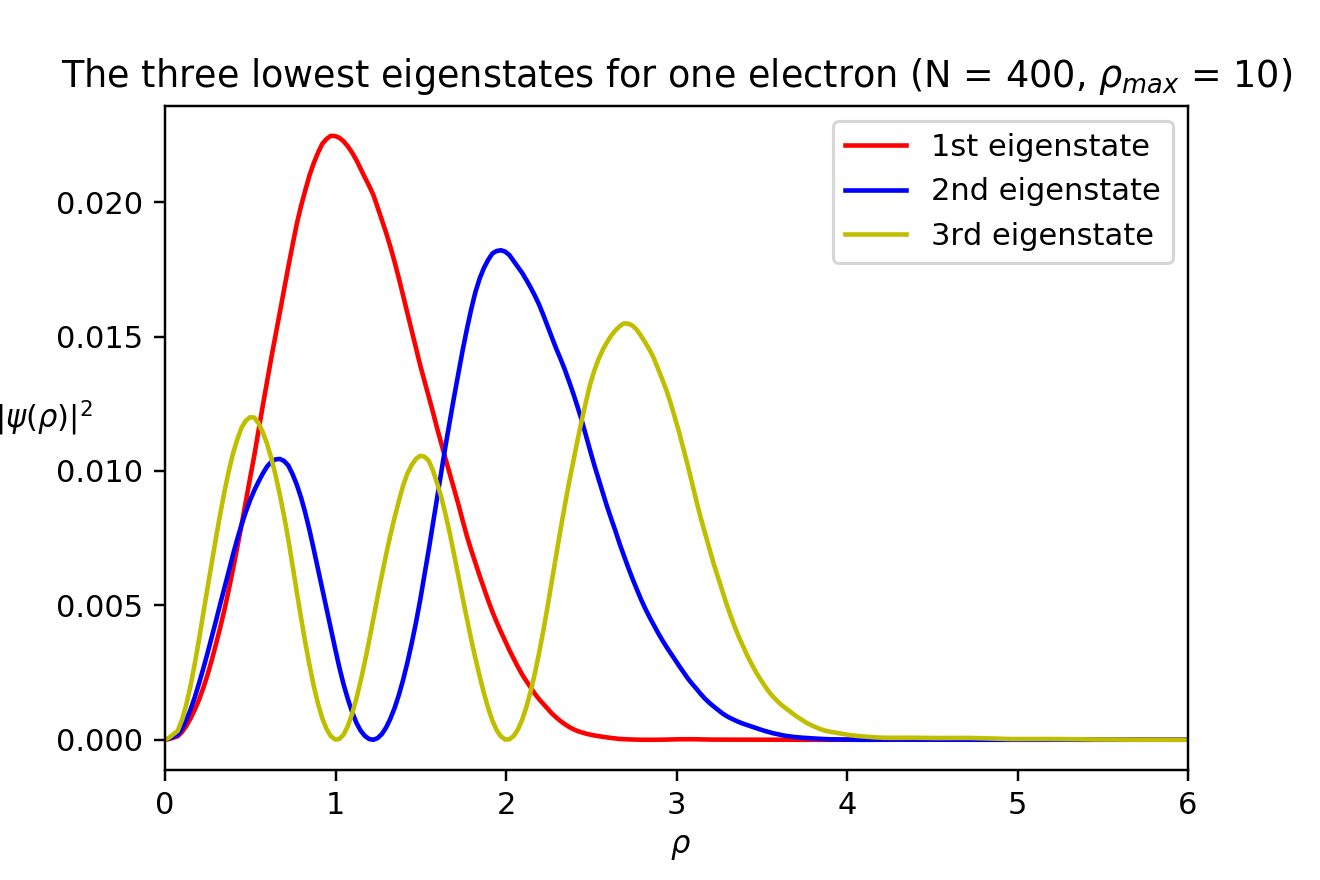
\includegraphics[scale=0.6]{three_lowest_one_e.png}
\end{figure}

\subsubsection{Number of iterations}
The number of similarity transformations needed to calculate the eigenvalues were logged by saving the number of iterations used in the algorithm for different number of grid points, N. The relationship can be seen in table (\ref{tab:iteratiation}).
\begin{table}[!h]
\centering
\caption{The number of iterations in the algorithm corresponds to the number of similarity transformations. To the right, the number of iterations can be seen with respect to the number of grid points, N. $\rho_{max}$ was set to 10. The number of iterations scales as $\approx 1.63N^{2}$.}
\label{tab:iteratiation}
\begin{tabular}{|l|l|}
\hline
\bf Grid points, N    &\bf Iterations\\ \hline
10       &  0  \\ \hline
150      &  36411   \\ \hline
400      &  268846  \\ \hline
500      &  422320  \\ \hline

\end{tabular}
\end{table}



\subsection{Choice of N and $\rho$}
The Jacobi algorithm gives the user the opportunity to increase the accuracy by changing the number of grid points, N, and the value of $\rho_{max}$. The algorithm was run for different values, and the calculated lowest eigenvalues were logged. The results are presented in table (\ref{tab:N_Rho_Lambda}).
\begin{table}[!h]
\centering
\caption{Different choices of N and $\rho_{max}$ influences the calculated eigenvalue.y.}
\label{tab:N_Rho_Lambda}
\begin{tabular}{|l|l|l|}
\hline
$\mathbf{\rho_{max}}$    &\bf Grid points, N &\bf Calculated $\mathbf{\lambda_0}$\\ \hline
1   & 10       & 10.0702\\ \hline
1  & 150        &  10.1508\\ \hline
1 & 400       &  10.1513\\ \hline
1 & 500      &  10.1511\\ \hline
10   & 10       & 2.68672\\ \hline
10  & 150        &  2.99861\\ \hline
10 & 400       &  2.9998\\ \hline
10 & 500      &  2.99987\\ \hline
20   & 10       & 4.49479\\ \hline
20  & 150        &  2.99443 \\ \hline
20 & 400       &  2.99922 \\ \hline
20 & 500      &  2.9995\\ \hline
\end{tabular}
\end{table}





\subsection{Two-electron system}
The square of the wave functions for the ground states of the two-electron system was found and plotted both with and without interaction. The new frequency $\omega$ was varied with the values $\omega = [0.01, 0.5, 1, 5]$. The plots can be seen in the figures (\ref{fig:two_001} - \ref{fig:two_5}). 

\begin{figure}[!h]
\centering
\caption{Plot of the square of the wave functions (ground state) for the two-electron system with and without interaction ($\omega = 0.01$). One can see that the wave functions span a large part of the $\rho$-axis. The difference between the interacting and non-interacting case is also relatively large.}
\label{fig:two_001}
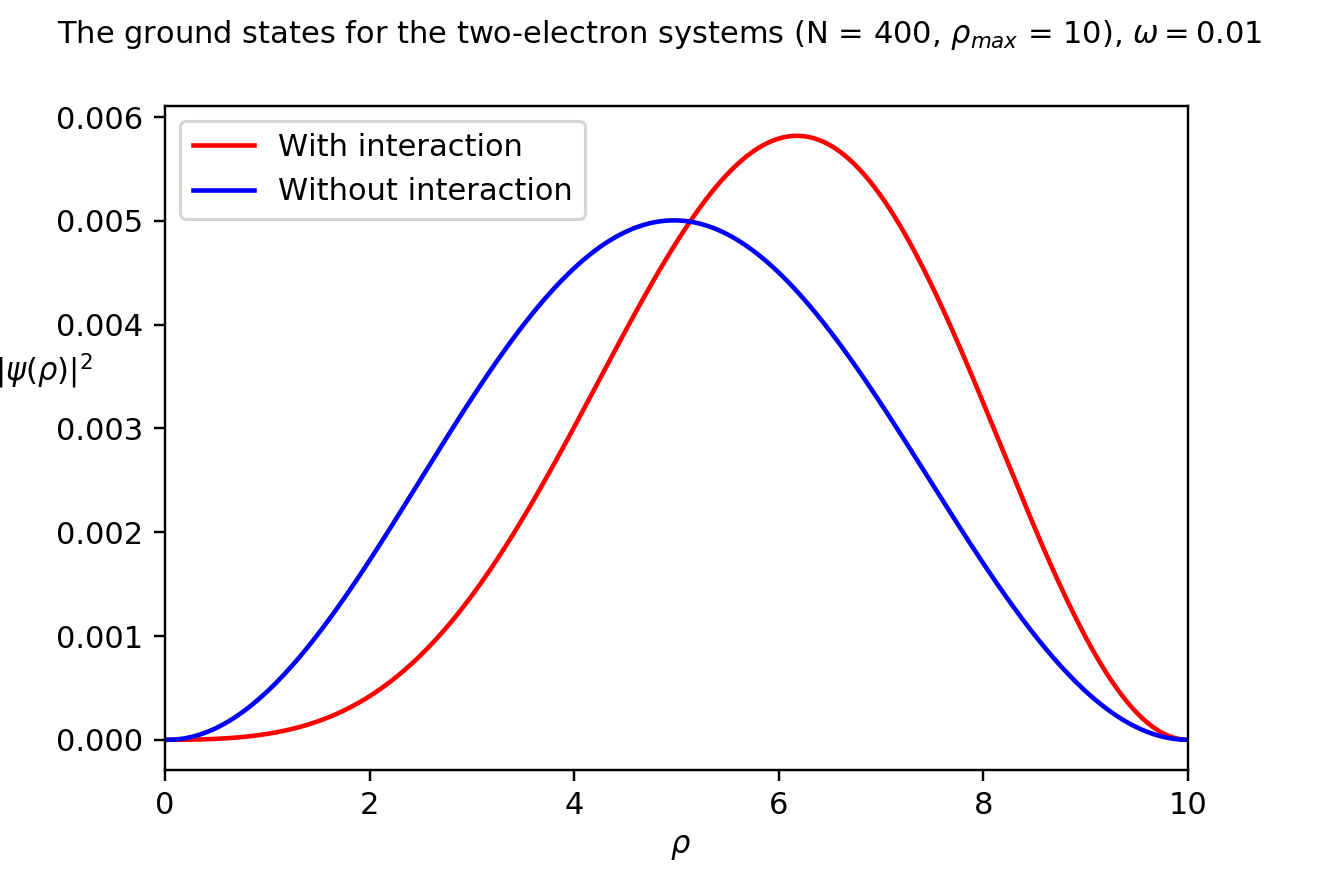
\includegraphics[scale=0.6]{non_vs_int_two_e_001.png}
\end{figure}

\begin{figure}[!h]
\centering
\caption{Plot of the square of the wave functions (ground state) for the two-electron system with and without interaction ($\omega = 0.5$). }
\label{fig:two_05}
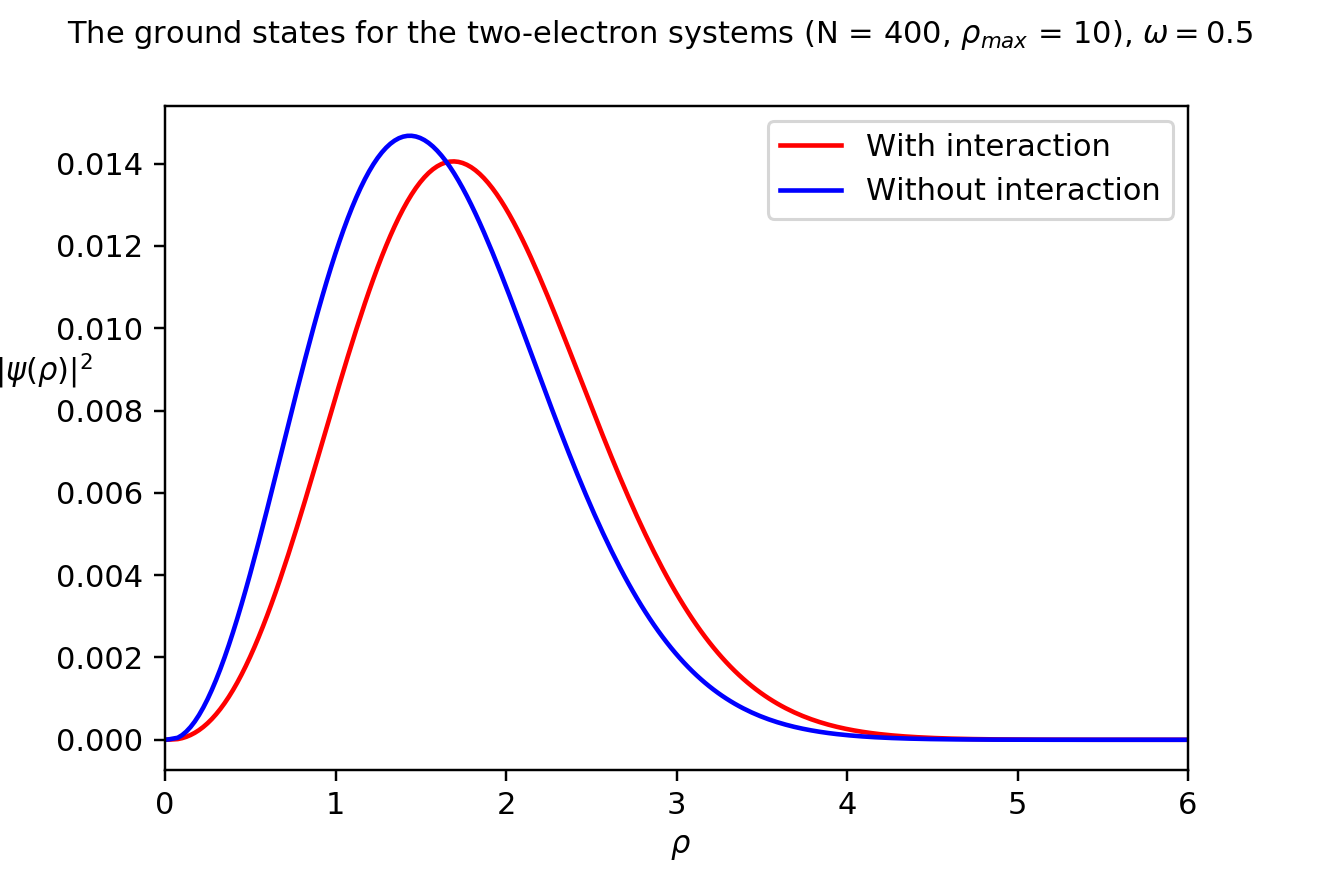
\includegraphics[scale=0.6]{non_vs_int_two_e_05.png}
\end{figure}

\begin{figure}[!h]
\centering
\caption{Plot of the square of the wave functions (ground state) for the two-electron system with and without interaction ($\omega = 1.0$).}
\label{fig:two_1}
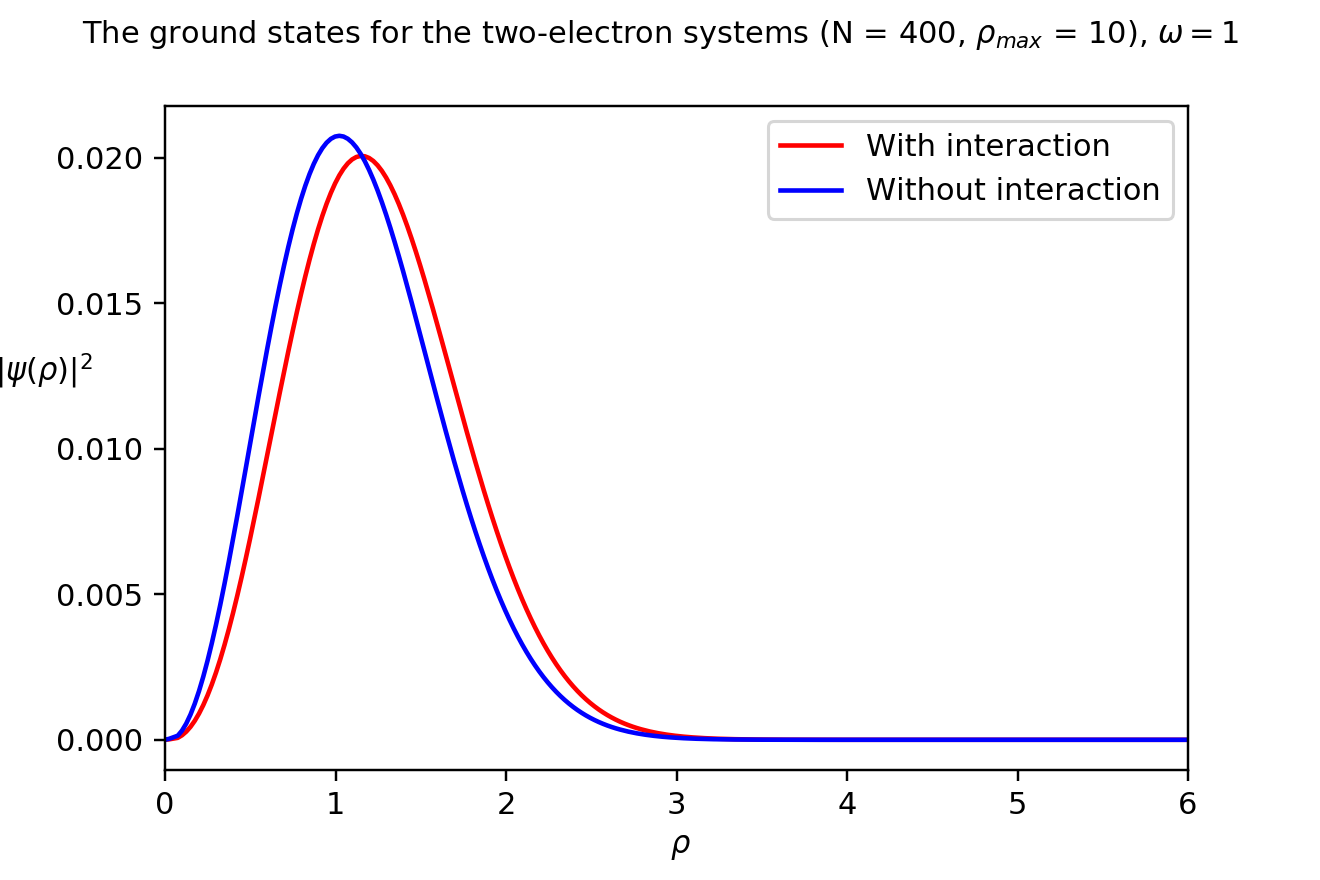
\includegraphics[scale=0.6]{non_vs_int_two_e_1.png}
\end{figure}

\begin{figure}[!h]
\centering
\caption{Plot of the square of the wave functions (ground state) for the two-electron system with and without interaction ($\omega = 5.0$). One can now see that the wave functions span a smaller part of the x-axis compared to the other figures. The difference between the interacting and non-interacting case is also smaller.}
\label{fig:two_5}
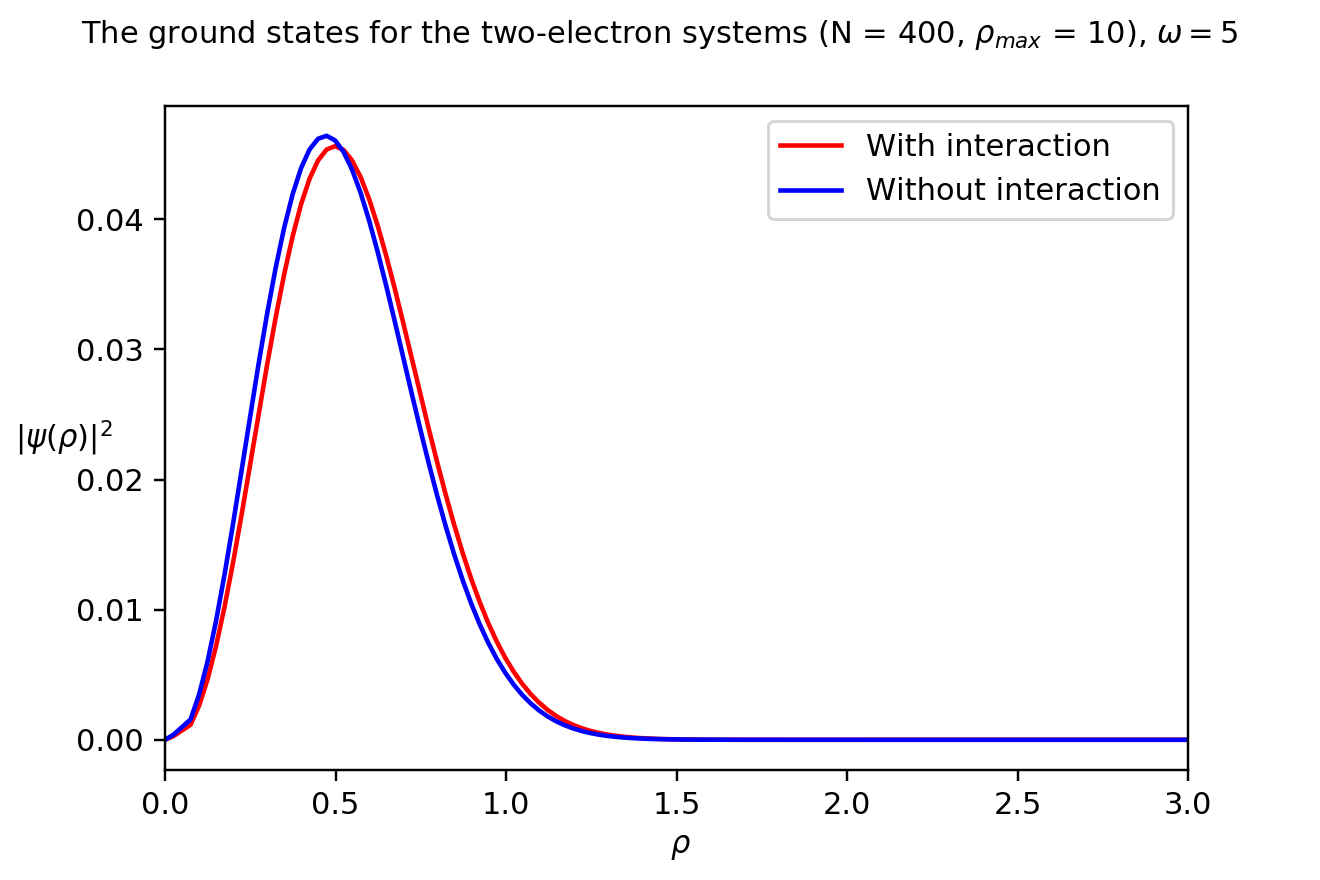
\includegraphics[scale=0.6]{non_vs_int_two_e_5.png}
\end{figure}


\subsection{Comparison to analytical solutions}
In table (\ref{tab:Analytical_vs}), the deviation from the analytical solutions for the one-electron case can be seen. The deviation is on the order of $10^{-4}$ to $10^{-3}$ for $N = 400$ and $\rho_{max} = 10$.

\begin{table}[]
\centering
\caption{The three first analytical eigenvalues compared to the numerical values.  The number of grid points, N, were set to 400, and $\rho_{max}$ was set to 10. The deviation is on the order of $10^{-4}$ to $10^{-3}$.}
\label{tab:Analytical_vs}
\begin{tabular}{|l|l|l|}
\hline
$\mathbf{\lambda_{Analytical}}$    & $\mathbf{\lambda_{Numerical}}$ &\bf Deviation\\ \hline
3   & 2.9998       & 0.0002\\ \hline
7  & 6.99902        &  0.00098\\ \hline
11 & 10.9976        &  0.0024\\ \hline
\end{tabular}
\end{table}



\section{Discussion}
In table (\ref{tab:Comptime}), one could see that the Jacobi method solver made in this project was considerably slower than the solver from the Armadillo library. The time also increased quite rapidly with increasing grid points compared to the Armadillo solver. This is probably because the FLOPS of the Jacobi solver scales with a higher order of N. 

In figure (\ref{fig:wave_one}), the one-electron wavefunctions were plotted. One can here see that by increasing the energy (going from the 1st eigenstate to the 2nd and 3rd), the wavefunctions spans over a larger part of the $\rho$, which implies a larger radius. Furthermore, going above the ground state increases the amount of local minima and maxima. This could resemble the behaviour of electrons in an atom. 

The three lowest eigenvalues were calculated with different number of grid points and values of $\rho_{max}$ to find a satisfying accuracy. $N=400$ and $\rho_{max}$ were found to be sufficient with a deviation on the order of $10^{-4}$ to $10^{-3}$. The deviations is shown in table (\ref{tab:Analytical_vs}), and confirms that the implemented Jacobi algorithm calculates the correct eigenvalues. 

The number of iterations (similarity transformations) as a function of grid points, N, was shown in table (\ref{tab:iteratiation}). It was found that the number of iterations scaled as $\approx 1.63\cdot N^{2}$. This explains the long computation times for large matrices. It is probably due to the part of the algorithm which checks for the largest element in the matrix. These types of operations scales with $N^{2}$. 

The two-electron wave functions were plotted for different values of $\omega$, and are shown in figures ((\ref{fig:two_001} - \ref{fig:two_5})). One can see that the waves becomes wider for larger values of $\omega$. This is due to the fact that a lower value of $\omega$ makes a weaker potential. It will thus make the distance between the two electrons large, explaining the behaviour seen in this project. 

In the same figures, one can also compare the interacting case with the non-interacting case. For larger values of $\omega$, the difference between the two cases becomes lower. This is because at the stronger potential at higher values of $\omega$, the kinetic energy of the electrons are higher, making the Couloumb interaction less important. 



\section{Conclusion}
In this project, it was shown that the Jacobi algorithm was much slower than the Armadillo algorithm used as a benchmark. This could be due to the fact that the implemented algorithm has to search through a matrix to find the highest element which is a time consuming operation. The algorithm could probably be improved by utilizing the fact that the matrix used is already tridiagonal. Next, the choice of the number of grid points and value of $\rho_{max}$ was shown to influence the accuracy and computation time of the algorithm. Lastly, it was also shown that the value $\omega$ affects the probability distribution of the position of the electron by changing the strength of the potential. The influence was found to be different for the interacting and non-interacting case. 




%-----------------------------------------------------%



\begin{flushleft}

\begin{thebibliography}{}

\singlespacing
\small




  
\bibitem{Article}
  Morten Hjorth-Jensen,
  Computational Physics,
  August 2015
  
\end{thebibliography}
\end{flushleft}



\end{document}




















